% !TEX program = lualatex
% !TEX encoding = utf8
\documentclass[german,colorful]{ExerciseLua}

\usepackage[
    unicode=true,
    pdftoolbar=false,
    pdfmenubar=false,
    pdffitwindow=true,
    pdfstartview=FitB,
    pdfauthor=SarsNeunSieben,
    pdfsubject=Übung
]{hyperref}
\usepackage{cleveref}

% \usepackage{lcg}
% \reinitrand[counter=sec,first=1,last=151]
% \usepackage[pages=all]{background}
% \backgroundsetup{
% scale=1,
% color=black,
% opacity=0.1,
% angle=0,
% contents={%
%     \rand\includegraphics[width=\textwidth]{~/PokemonGen1/\arabic{sec}.png}
%     }%
% }

\usepackage{tikz}
\usetikzlibrary{arrows.meta,positioning,calc,automata,quotes}
\tikzstyle{vertex}=[draw,fill=black!15,circle,minimum size=20pt,inner sep=0pt]
\tikzset{
    old inner xsep/.estore in=\oldinnerxsep,
    old inner ysep/.estore in=\oldinnerysep,
    double circle/.style 2 args={
        circle,
        old inner xsep=\pgfkeysvalueof{/pgf/inner xsep},
        old inner ysep=\pgfkeysvalueof{/pgf/inner ysep},
        /pgf/inner xsep=\oldinnerxsep+#1,
        /pgf/inner ysep=\oldinnerysep+#1,
        alias=sourcenode,
        append after command={
        let     \p1 = (sourcenode.center),
                \p2 = (sourcenode.east),
                \n1 = {\x2-\x1-#1-0.5*\pgflinewidth}
        in
            node [inner sep=0pt, draw, circle, minimum width=2*\n1,at=(\p1),#2] {}
        }
    },
    double circle/.default={2pt}{black},
    zielknoten/.style={draw=emorot,line width=.75mm,circle,minimum size=2em,inner sep=0pt},
    startknoten/.style={draw=betterGreen,line width=.75mm,circle,minimum size=2em,inner sep=0pt}
}

%%%%%%%%%%%%%%%%%%%%%%%%%%%%%%%%%%%%%%%%%%%%%%%%%%%%%%%%%%%%%%%%%%%%%%%%%%%%
% Defines for mathematical notation. Add additional defines as needed.
%%%%%%%%%%%%%%%%%%%%%%%%%%%%%%%%%%%%%%%%%%%%%%%%%%%%%%%%%%%%%%%%%%%%%%%%%%%%
\newcommand{\N}{\ensuremath{\mathbb{N}}}% natural number
\newcommand{\Z}{\ensuremath{\mathbb{Z}}}% whole numbers
\newcommand{\R}{\ensuremath{\mathbb{R}}}% real numbers
\newcommand{\Q}{\ensuremath{\mathbb{Q}}}% rational numbers
\newcommand{\C}{\ensuremath{\mathbb{C}}}% complex numbers
%%%%%%%%%%%%%%%%%%%%%%%%%%%%%%%%%%%%%%%%%%%%%%%%%%%%%%%%%%%%%%%%%%%%%%%%%%%%

\setLecture[KI]{{\color{goetheblau}Einführung in die Methoden der Künstlichen Intelligenz}}
\setSemester{Sommer 2022}

\setName{SarsNeunSieben}
\setStdID{1234567}
\setGroup{1}
\setAssignment{2}

\begin{document}
    \begin{exercise}{1}
        \begin{enumerate}[label=\alph*)]
            \item Wir beginnen mit dem Startknoten {\color{betterGreen}$(0,0)$} und können die Zielknoten {\color{emorot}$(1,0)$} und {\color{emorot}$(2,1)$} erreichen.
            \begin{center}
              \begin{tikzpicture}[>=Stealth, auto,
                node distance = 2*\dis, on grid,
                every state/.style = {circle, draw, very thick, minimum size=2em, inner sep=0pt},
                every edge/.style = {draw, semithick, -Stealth, shorten >=1pt},
                every edge quotes/.style = {sloped, font=\small}]
                \def\dis{1cm}
                \begin{scope}[nodes=state]
                    \node (s) [startknoten] {$(0,0)$};
                    \node (20) [below of=s] {$(2,0)$};
                    \node (01) [left of=20] {$(0,1)$};

                    \node (11) [below of=20] {$(1,1)$};
                    \node (21) [zielknoten,left of=11] {$(2,1)$};
                \end{scope}
                \node (10) [zielknoten,right of=20] {$(1,0)$};
                \path (s) edge (01)
                    (s) edge (20)
                    (s) edge (10)

                    (01) edge (21)
                    (01) edge (11)
                    (01) edge (s)

                    (10) edge (s)
                    (10) edge (20)
                    (10) edge (11)
                    
                    (20) edge (21)
                    (20) edge (10)
                    (20) edge (s)
                    
                    (11) edge (01)
                    (11) edge (21)
                    (11) edge (10)
                    
                    (21) edge (01)
                    (21) edge (20)
                    (21) edge (11);
              \end{tikzpicture}
            \end{center}
            \item Wir betrachten zunächst nur das $y$. Dafür haben wir insgesamt $n$ Möglichkeiten, wobei der erste Fall $y=0$ ein Sonderfall ist, genau so wie $y=n-1$. Damit haben wir $n-2$ Möglichkeiten für $y$ um in den letzten Fall zu kommen. Dazu kommt noch, dass wir für das $x$ $m$ verschieden Möglichkeiten haben, da wir in allen Formel das $x$ nur dann erhöhen, wenn wir es auch $\mod m$ nehmen. Somit haben wir $\left(\left(n - 2\right) \cdot m\right) \cdot 4$ Nachfolger durch den letztem Fall. Zusätzlich haben wir 2 Sonderfälle für $y=0$ und $y=n-1$, wobei wir hier je 3 Nachfolger haben, und wieder $m$ Möglichkeiten für $x$. Dies ist addiert nun die Gesamtanzahl der Kanten, wenn Zielknoten auch Kanten haben. \\
            Um den mittleren Verzweigungsgrad zu erhalten teilen wir nun diese Summe durch die Gesamtzahl der Knoten. Die Gesamtzahl der Knoten ist $m \cdot n$, da wir durch die Formeln beginnend mit $0$ sowohl $x$ als auch $y$ bis $m$ bzw. $n$ schrittweise um 1 erhöhen, wodurch alle Knoten bis $(m,n)$ erreicht werden können.
            \[\text{mittlerer Verzweigungsgrad} = \frac{\overbrace{\left(\left(n - 2\right) \cdot m\right) \cdot 4}^{\text{unterste Formel}} + \overbrace{\left(2 \cdot m\right) \cdot 3}^{\text{Sonderfälle}}}{\underbrace{m \cdot n}_{\text{Gesamtzahl der Knoten}}} \]
            \pagebreak\item Der Knoten mit {\color{betterGreen}grünem} Rahmen ist der Startknoten, die Knoten mit {\color{emorot}rotem} Rahmen sind Zielknoten.
            \begin{enumerate}
                \item[\color{olive}1F1] = 1. Funktion 1. Parameter, also $(x,y+1)$
                \item[\color{betterGreen}{3F2}] = 3. Funktion 2. Parameter, also $(x,y+1)$
                \item[\color{teal}{2F1}] = 2. Funktion 1. Parameter, also $((x-1) \mod m, y)$
                \item[\color{blue}2F3] = 2. Funktion 3. Parameter, also $(x,y-1)$
                \item[\color{emorot}3F1] = 3. Funktion 1. Parameter, also $(x, y-1)$
                \item[{\color{pink}*}] = falls $x=n$ und $y=n-1$, sodass dies ein Zielknoten ist
                \end{enumerate}
                Die Tiefensuche mit Sharing ist in diesem Fall unabhängig von $m$ und $n$ und findet immer den Zielknoten $(1,0)$, wie in unserem Beispiel gezeigt.
                \begin{center}
                \begin{tikzpicture}[>=Stealth, auto,
                    node distance = 2*\dis, on grid,
                    every state/.style = {circle, draw, very thick, minimum size=2em, inner sep=0pt},
                    every edge/.style = {draw, semithick, -Stealth, shorten >=1pt},
                    every edge quotes/.style = {sloped, font=\small},
                    descr/.style={sloped}]
                    \def\dis{1.5cm}
                    \begin{scope}[nodes=state]
                        \node (00) [startknoten] at (0,0) {$(0,0)$};
                        \node (01) [below of=00] {$(0,1)$};
                        \node (1) [below of=01] {$\vdots$};
                        \node (0n2) [below of=1] {$(0,n-2)$};
                        \node (0n1) [below of=0n2] {$(0,n-1)$};

                        \node (m1n1) [right of=0n1] {$(m-1,n-1)$};
                        \node (2) [right of=m1n1] {$\cdots$};
                        \node (nn1) [above of=2,zielknoten] {$(n,n-1)$};
                        \node (2n1) [right of=2] {$(2,n-1)$};
                        
                        \node (1n1) [right of=2n1] {$(1,n-1)$};
                        \node (1n2) [above of=1n1] {$(1,n-2)$};
                        \node (1n3) [above of=1n2] {$(1,n-3)$};
                        \node (3) [above of=1n3] {$\vdots$};
                        \node (10) [above of=3,zielknoten] {$(1,0)$};
                    \end{scope}
                    \path (00) edge[olive] node[descr] {1F1} (01)
                        (01) edge[betterGreen] node[descr] {3F2} (1)
                        (1) edge[betterGreen] node[descr] {3F2} (0n2)
                        (0n2) edge[betterGreen] node[descr] {3F2} (0n1)
                        (0n1) edge[teal] node[descr] {2F1} (m1n1)
                        (2) edge[pink] node[descr] {*} (nn1)
                        (m1n1) edge[teal] node[descr] {2F1} (2)
                        (2) edge[teal] node[descr] {2F1} (2n1)
                        (2n1) edge[teal] node[descr] {2F1} (1n1)
                        (1n1) edge[blue] node[descr] {2F3} (1n2)
                        (1n2) edge[emorot] node[descr] {3F1} (1n3)
                        (1n3) edge[emorot] node[descr] {3F1} (3)
                        (3) edge[emorot] node[descr] {3F1} (10);
                \end{tikzpicture}
            \end{center}
            \item Auch hier ist der Startknoten {\color{betterGreen}grün} markiert, und der Zielknoten {\color{emorot}rot}.\\

            Tiefensuche ohne Sharing terminiert nur für $n=2$, da wir nur so zur zweiten Formel kommen, ohne die dritte ausführen zu müssen. Denn in der zweiten Formel besuchen wir nie bekannte Knoten, sondern stets neue Knoten, wodurch wir einen Zielknoten erreichen werden.

            Die Suche terminiert nicht für $n>2$, da wir in der dritten Formel wieder unseren Startknoten besuchen und somit in eine Schleife kommen.
            \begin{center}
                \begin{tikzpicture}[>=Stealth, auto,
                    node distance = 2*\dis, on grid,
                    every state/.style = {circle, draw, very thick, minimum size=2em, inner sep=0pt},
                    every edge/.style = {draw, semithick, -Stealth, shorten >=1pt},
                    every edge quotes/.style = {sloped, font=\small},
                    descr/.style={sloped}]
                    \def\dis{1cm}
                    \begin{scope}[nodes=state]
                        \node (a00) [startknoten] at (0,0) {$(0,0)$};
                        \node (a01) [right of=a00] {$(0,1)$};
                        \node (a21) [right of=a01,zielknoten] {$(2,1)$};

                        \node (b00) [startknoten] at (7,1) {$(0,0)$};
                        \node (b01) [below of=b00] {$(0,1)$};
                    \end{scope}
                    \node () [below=1cm of a01] {terminiert für $n=2$};
                    \node () [below=1cm of b01] {terminiert nicht für $n>2$};
                    \path (a00) edge (a01)
                        (a01) edge (a21)
                        (b00) edge[in=135,out=225] (b01)
                        (b01) edge[in=-45,out=45] (b00);
                \end{tikzpicture}
            \end{center}
        \end{enumerate}
    \end{exercise}\pagebreak
    \begin{exercise}{2}
        Wir beginnen bei Knoten {\color{betterGreen}0} und unser Zielknoten ist {\color{emorot}2} in Tiefe 2.\\
        Da die Breitensuche zuerst in die Breite geht, und wir hier unendliche Breite haben, wird diese hier nie terminieren, obwohl es einen endlichen Pfad gäbe.
        \begin{center}
            \begin{tikzpicture}[every node/.style = {circle, draw, very thick, minimum size=2em, inner sep=0pt}]
                \node (0) [startknoten] {$0$}
                    child {
                        node {$1$}
                        child {
                            node [zielknoten] {$2$}
                        }
                    }
                    child {
                        node {$3$}
                    }
                    child {
                        node {$\ldots$}
                    }
                    child {
                        node {$\infty$}
                    };
            \end{tikzpicture}
        \end{center}
    \end{exercise}
    \begin{exercise}{3}
        Die Zahl besagt die Schritt-Nummer, wobei {\color{orange}orange} dem {\color{orange}Bergsteigen} entspricht und {\color{blue}blau} der {\color{blue}Best-First Suche} entspricht.\\
        Die Best-First Suche wählt bei mehreren Kindern in der Tiefe 1 zuerst den rechten Knoten, dann den linken. In allen anderen Tiefen wird zuerst das linke Kind genommen.\\
        Das Bergsteigen wählt immer zuerst das rechte Kind aus.
        \begin{center}
            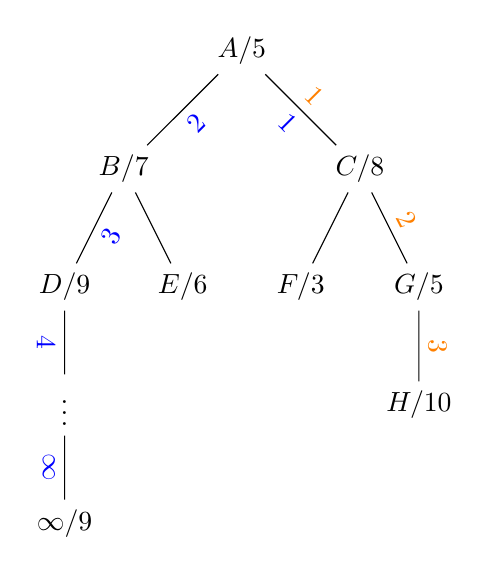
\begin{tikzpicture}
                \node(a) {$A/5$}
                    child {
                        node {$B/7$} 
                        child {
                            node {$D/9$}
                            child {
                                node {$\vdots$}
                                child {
                                    node {$\infty/9$}
                                    edge from parent node [sloped,below,blue] {$\infty$}
                                }
                                edge from parent node [sloped,below,blue] {$4$}
                            }
                            edge from parent node [sloped,below,blue] {3}
                        }
                        child {
                            node {$E/6$}
                        }
                        edge from parent [black] node [sloped,below,blue] {2}
                    }
                    child[missing]
                    child {
                        node {$C/8$}
                        child {
                            node {$F/3$}
                        }
                        child {
                            node {$G/5$}
                            child {
                                node {$H/10$}
                                edge from parent node [sloped,above,orange] {3}
                            }
                            edge from parent node [sloped,above,orange] {2}
                        }
                        edge from parent node [sloped,below,blue] {1} node [sloped,above,orange] {1}
                        };
            \end{tikzpicture}
        \end{center}
        Best-First will zuerst den linken Teilbaum komplett abgehen, da der Knoten $B$ weniger Gewicht hat, und somit diesen Teilbaum zuerst betrachtet. \\
        Bergsteigen wiederum betrachtet zuerst den Teilbaum, in den er zuerst gegangen ist. Dadurch kann dieser auch in diesem Fall terminieren.
    \end{exercise}
\end{document}
